\documentclass[letterpaper,twocolumn,10pt]{article}

% Venue-neutral two-column review layout.
\usepackage[utf8]{inputenc}
\usepackage[T1]{fontenc}
\usepackage{times}
\usepackage[margin=0.72in]{geometry}
\usepackage{amsmath,amssymb}
\usepackage{bm}
\usepackage{graphicx}
\usepackage{booktabs}
\usepackage{algorithm}
\usepackage{algorithmic}
\usepackage{hyperref}
\usepackage{cite}
\setlength{\columnsep}{0.24in}
\graphicspath{{figures/}}

\title{CREATE: Closed-Loop Reward Evolution via Training--Evaluation Feedback}

\author{Anonymous Authors}

\begin{document}

\maketitle

\begin{abstract}
Evaluating a candidate reward function requires training a reinforcement learning policy to completion, making policy training the dominant cost in LLM-based reward search. Existing multi-candidate methods allocate this budget to breadth---generating many candidates, training a policy for each, and selecting the best---using completed training runs primarily to rank candidates while discarding rich per-component diagnostic signals. We study a complementary budget allocation: iteratively repair one active reward lineage using structured evidence from each training run.
We propose CREATE (Closed-loop Reward Evolution Agent with Training--Evaluation Feedback), which organizes component-level activation rates, magnitude distributions, development-evaluation outcomes, and lineage modification history into an auditable failure diagnosis, then applies a severity-gated edit---parameter tuning, component refactoring, or structural redesign---along the same reward lineage. Each local edit targets one component, producing an auditable sequence of one modification, one training run, and one observed feedback signal.
On LunarLander-v3 across five independent search paths, all five initially sub-threshold reward functions are repaired to surpass the 200-point threshold within ten iterations (development $228.98 \pm 16.54$), and the repaired rewards generalize to held-out evaluation seeds unseen during search ($231.63 \pm 12.23$ over 100 episodes). Under a matched per-evaluation training budget and common ten-evaluation cap, iterative single-lineage repair reaches 5/5 while budget-equivalent independent generation reaches 0/5 (50 policy trainings versus 33 with early stopping). On BipedalWalker-v3, all five lineages reach the 300-point threshold (held-out $310.82 \pm 5.03$), including a repair from 103.03 to 304.92. An exploratory Ant-v4 run ($-12.04 \rightarrow 1414.47$) demonstrates pipeline feasibility in a high-dimensional continuous-control setting.
\end{abstract}

\section{Introduction}

Reward functions translate task goals into optimization signals for reinforcement learning (RL) agents. A well-designed reward function provides dense, well-scaled feedback that guides the agent toward task completion. A poorly designed one produces agents that exploit loopholes, converge to local optima, or fail to learn entirely \cite{ng1999policy,singh2010intrinsically}. Traditional reward engineering requires domain experts to cycle through reward design, policy training, behavior observation, and parameter tuning---a labor-intensive, trial-and-error process that has resisted automation.

Large language models (LLMs) can generate executable reward code from natural language task descriptions and environment interfaces \cite{eureka,text2reward,language2rewards}. This capability has catalyzed a shift from one-shot reward generation to reward \emph{search}: methods now generate multiple reward candidates, train a policy for each, and select the best-performing one. Evolutionary search \cite{eureka}, tree-structured exploration \cite{rfagent}, and agent-based iteration \cite{card,rda} have all demonstrated that systematic exploration of the reward design space improves over single-shot generation.

However, reward code generation is often cheaper than evaluating the resulting code. Each candidate evaluation requires training a policy for hundreds of thousands to millions of environment interactions. In multi-candidate search pipelines, substantial training budget may be consumed by candidates that are ultimately not selected. A completed training run, even a failed one, is nevertheless informative: it exposes per-component activation rates and magnitude distributions, episode length and termination statistics, and reward code runtime errors. Most candidate-selection pipelines reduce this evidence to a scalar evaluation score and discard the rest.

A training run that consumed a million environment steps produced data. Can that data be used to \emph{repair} the reward function that produced it, rather than merely to score and discard it? This question motivates our work.

Na\"ively asking an LLM to rewrite a reward function based on the final score alone does not reliably solve this problem. Two issues arise. First, a scalar score lacks diagnostic precision: it cannot distinguish between a progress reward whose weights need tuning, a stability term whose mathematical form is inappropriate, and an overall structure that is fundamentally misaligned with the task. Second, when an LLM modifies multiple reward components simultaneously, the resulting score change cannot be attributed to any specific edit---the agent receives a compound outcome with no way to determine which modification was beneficial, neutral, or harmful.

These issues point to two design requirements for iterative reward repair. First, training feedback should decompose outcomes at the component level, so that failure can be diagnosed with sufficient precision to identify a specific editing target. Second, local editing should be constrained to one target component per iteration, yielding an auditable sequence of one modification, one training run, and one observed feedback signal.

We propose CREATE (Closed-loop Reward Evolution Agent with Training--Evaluation Feedback), which iteratively repairs a single reward lineage through structured evidence diagnosis and severity-gated editing. CREATE initializes a reward program from the task interface, then iterates through training, evaluation, evidence assembly, failure diagnosis, and targeted editing. A Best Archive preserves the historically best reward--policy pair, allowing the active lineage to explore edits that may temporarily reduce performance without losing accumulated progress.

Our contributions are as follows:
\begin{enumerate}
    \item We propose CREATE, a feedback-driven iterative reward refinement framework that combines three mechanisms: (i)~component-level reward evidence that exposes activation patterns, magnitude distributions, and termination behavior at the granularity of individual reward terms; (ii)~auditable failure diagnosis that maps this evidence to a primary failure hypothesis and a specific editing target; and (iii)~a severity-gated edit controller that selects among parameter tuning, component refactoring, or structural redesign according to problem severity, and constrains each local edit to one component.
    \item Across five independent search paths on LunarLander-v3, all five initially sub-threshold reward functions are repaired to surpass the 200-point threshold. Under a matched per-evaluation training budget, iterative single-lineage repair reaches 5/5 while budget-equivalent independent generation reaches 0/5. On BipedalWalker-v3, all five lineages reach the 300-point threshold, including a repair from 103.03 to 304.92.
\end{enumerate}

\section{Related Work}

\subsection{Classical Reward Design}

Reward shaping augments the environment reward with auxiliary signals to accelerate learning. Potential-based reward shaping \cite{ng1999policy,wiewiora2003potential} provides theoretical guarantees that specific reward transformations preserve the optimal policy. Inverse reinforcement learning \cite{ng2000algorithms,abbeel2004apprenticeship,ziebart2008maximum} infers reward functions from expert demonstrations rather than manual specification. These approaches reduce but do not eliminate human effort: practitioners must still provide shaping structures, potential functions, task decompositions, or demonstration data.

\subsection{LLM-Based Reward Generation and Search}

Large language models can generate executable reward code from task descriptions, environment interfaces, and available sensor signals. Eureka \cite{eureka} pioneered LLM-driven evolutionary reward search, combining code generation with reward reflection across 29 IsaacGym tasks and demonstrating human-level reward design on 83\% of them. Text2Reward \cite{text2reward} generates dense reward programs from natural language descriptions. Language to Rewards \cite{language2rewards} uses a two-stage pipeline that translates task goals into natural language motion plans, then into reward code for real-robot deployment.

Subsequent work has expanded the search paradigm. CARD \cite{card} introduces trajectory preference evaluation to reduce per-iteration training cost. RF-Agent \cite{rfagent} frames reward design as sequential decision-making with Monte Carlo tree search. REvolve \cite{revolve} incorporates human feedback through Elo ratings. STRIDE \cite{stride} demonstrates an agentic engineering pipeline for humanoid locomotion. RDA \cite{rda} leverages vision-language models to evaluate trajectory--task alignment. CoUR \cite{cour} uses Bayesian decoupling for modular reward optimization.

The dominant strategy across these methods is breadth-oriented: generate many candidates, train policies for all, and select the best. Per-component diagnostic signals from candidates that are not selected---their activation patterns, magnitude ratios, and termination modes---are discarded with the scalar score.

\subsection{Diagnostic-Driven Reward Refinement}

A parallel line of work treats reward design as iterative debugging rather than one-shot generation or population-based selection. Self-Refined reward design \cite{selfrefine} uses LLM-internal code-level reflection without environment interaction. Self-correcting reward shaping \cite{selfcorrecting} adjusts scalar weights in a closed loop but provides only aggregate performance feedback. Most relevant to our work, diagnostic-driven refinement for discrete grid tasks \cite{wang2026diagnostic} identifies a taxonomy of failure modes and uses budget-matched comparisons, demonstrating the value of structured diagnosis in a simplified setting.

CREATE extends the diagnostic-driven approach in three ways. First, it operates on standard continuous-control benchmarks (LunarLander, BipedalWalker, Ant) rather than discrete grid worlds. Second, it introduces a severity-gated edit controller: parameter tuning, component refactoring, and structural redesign are applied at graduated levels of intervention rather than as a uniform operation. Third, it enforces a single-component editing constraint that makes each modification individually auditable---one edit, one training run, one observed outcome. The dominant multi-candidate search paradigm allocates budget to breadth; CREATE allocates it to depth. Where tree-based search pursues structural diversity \cite{rfagent}, CREATE pursues diagnostic precision along one lineage.

\section{Method}

Figure~\ref{fig:framework} presents the system architecture. CREATE operates as a closed loop: a reward program is used to train a policy; the trained policy is evaluated on the environment's native objective; per-component training traces, development outcomes, and lineage history are assembled into structured evidence; a failure diagnosis identifies the primary problem and a specific editing target; and a severity-gated edit controller selects an intervention level and produces the next reward. Generated rewards feed policy training exclusively; the environment's native reward is reserved for development evaluation.

\begin{figure*}[t]
\centering
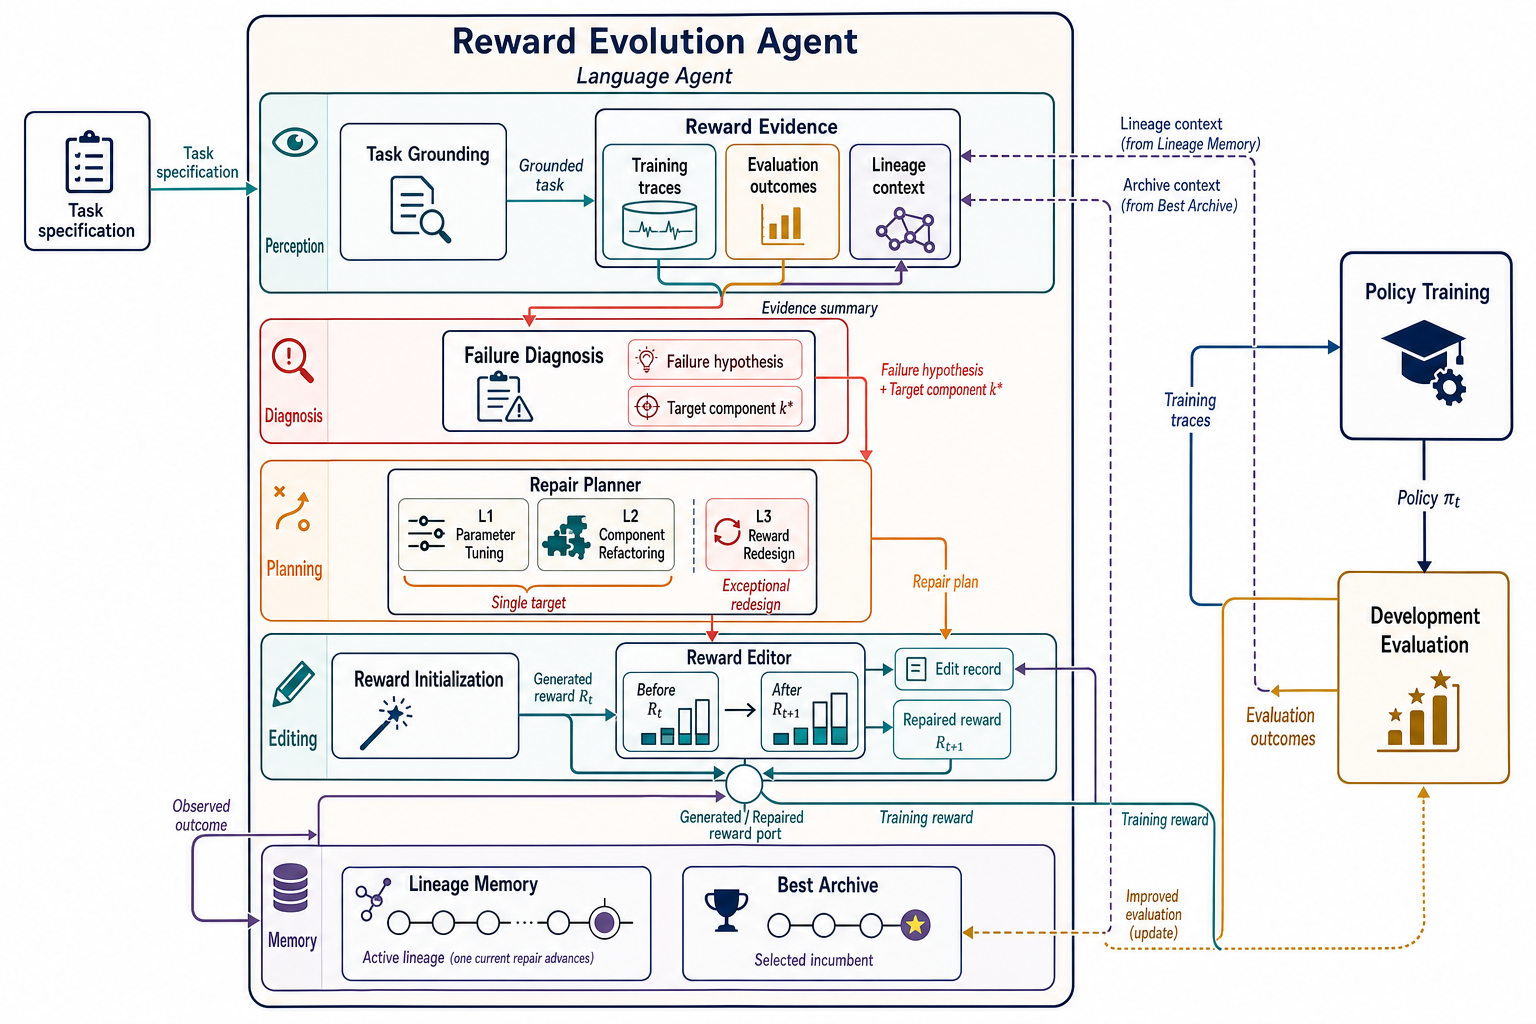
\includegraphics[width=0.98\textwidth]{reward_evolution_agent_framework.png}
\caption{Overview of CREATE. Training traces, development-evaluation outcomes, and lineage context are combined as reward evidence. The edit controller selects among parameter tuning, component refactoring, or structural redesign based on problem severity. Each local edit targets one component. A Best Archive preserves the historically best reward--policy pair.}
\label{fig:framework}
\end{figure*}

\subsection{Problem Formulation and Budget Model}

Let $\mathcal{E}$ be a reinforcement learning environment with state space $\mathcal{S}$, action space $\mathcal{A}$, and native reward function $r_{\text{env}}: \mathcal{S} \times \mathcal{A} \times \mathcal{S} \rightarrow \mathbb{R}$. A task interface $I$ provides the observation and action schemas, available sensor signals, and a natural-language task description. The learner has access to a single policy-training budget $B$ (environment steps per reward evaluation) and a maximum number of reward evaluations $K$.

At iteration $t$, a reward program $R_t$ maps transitions to scalar training rewards:
\begin{equation}
r_{\text{gen},t}^{(k)} = R_t(s_k, a_k, s_{k+1}).
\label{eq:gen_reward}
\end{equation}
Policy training uses $r_{\text{gen},t}$ as the exclusive learning signal:
\begin{equation}
(\pi_t, \mathcal{T}_t) = \text{PolicyTrain}(\mathcal{E}, R_t; B),
\label{eq:policy_train}
\end{equation}
where $\pi_t$ is the trained policy and $\mathcal{T}_t$ records per-component reward statistics, episode lengths, termination information, and runtime errors accumulated during training.

After training, a development evaluator creates an unwrapped copy of the environment that exposes the native reward $r_{\text{env}}$. For each of $N$ fixed evaluation episodes, it computes the undiscounted cumulative native return:
\begin{equation}
G_{\text{env},t,i} = \sum_{k=0}^{H_i-1} r_{\text{env}}(s_k, a_k, s_{k+1}).
\label{eq:dev_return}
\end{equation}
The development score is the mean over evaluation episodes:
\begin{equation}
s_t = J_{\text{dev}}(\pi_t) = \frac{1}{N}\sum_{i=1}^{N} G_{\text{env},t,i}.
\label{eq:dev_score}
\end{equation}
The reward channels are kept separate:
\begin{equation}
\begin{aligned}
r_{\text{gen},t} &\rightarrow \text{Policy Optimization},\\
r_{\text{env}} &\rightarrow \text{Development Evaluation}.
\end{aligned}
\label{eq:dual_channel}
\end{equation}
This separation prevents the feedback loop from optimizing against its own evaluation metric.

An independent candidate search generates $K$ reward functions without inter-candidate information flow:
\begin{equation}
\mathcal{R}_{\text{ind}} = \{R^{(1)}, R^{(2)}, \ldots, R^{(K)}\}.
\label{eq:ind_search}
\end{equation}
In contrast, CREATE maintains a single active lineage:
\begin{equation}
R_1 \rightarrow R_2 \rightarrow \cdots \rightarrow R_K,
\label{eq:seq_path}
\end{equation}
where $R_{t+1}$ is produced by editing $R_t$ based on the training and evaluation feedback from iteration $t$. When each reward function is evaluated with $B$ environment steps of policy training, the cumulative budget after $n$ evaluations is identical for both paradigms:
\begin{equation}
C(n) = nB.
\label{eq:budget}
\end{equation}
Equation~\ref{eq:budget} defines equality at a fixed number $n$ of completed reward evaluations. In the experiments, both methods share the same per-evaluation cost and maximum $K$; early stopping means their realized total training costs need not be equal.

\subsection{Component-Level Evidence and Structured Diagnosis}

A scalar development score $s_t$ indicates whether the current policy reaches the task objective. It does not, by itself, indicate \emph{why} the reward function failed. To support targeted editing, CREATE decomposes training outcomes into per-component diagnostics.

Let the generated reward at iteration $t$ consist of $M_t$ named components:
\begin{equation}
r_{\text{gen},t}^{(k)} = \sum_{j=1}^{M_t} r_{t,j}^{(k)}.
\label{eq:components}
\end{equation}
For each component $j$, we compute three statistics from the training run. The mean per-episode cumulative return of component $j$:
\begin{equation}
\mu_{t,j} = \frac{1}{N_{\text{tr}}}\sum_{e=1}^{N_{\text{tr}}}\sum_{k=0}^{H_e-1} r_{t,j}^{(e,k)}.
\label{eq:mu}
\end{equation}
The activation rate---the fraction of environment steps in which component $j$ produces a non-negligible signal:
\begin{equation}
a_{t,j} = \frac{\sum_{e,k} \mathbb{I}(|r_{t,j}^{(e,k)}| > \varepsilon)}{\sum_e H_e}.
\label{eq:activation}
\end{equation}
The magnitude share---component $j$'s contribution relative to the total reward magnitude:
\begin{equation}
m_{t,j} = \frac{\sum_{e,k}|r_{t,j}^{(e,k)}|}{\sum_{\ell=1}^{M_t}\sum_{e,k}|r_{t,\ell}^{(e,k)}| + \varepsilon}.
\label{eq:magnitude}
\end{equation}

These statistics answer distinct diagnostic questions. Activation rate asks: \emph{does this component fire?} A near-zero activation rate accompanied by early termination suggests the component's triggering condition is too narrow---for instance, a sparse landing bonus that rarely activates. Magnitude share asks: \emph{does this component dominate the signal?} A component with high magnitude share but low activation may represent a large sparse bonus that overwhelms dense shaping terms. Mean cumulative return asks: \emph{what does this component contribute in absolute terms?}

The structured evidence $\mathcal{E}_t$ combines three information sources:
\begin{equation}
\mathcal{E}_t = (\mathcal{T}_t, \mathcal{D}_t, \mathcal{M}_{t-1}),
\label{eq:feedback}
\end{equation}
where $\mathcal{T}_t$ contains the per-component statistics (Eqs.~\ref{eq:mu}--\ref{eq:magnitude}), episode length distributions, termination and truncation counts, and code runtime errors; $\mathcal{D}_t$ contains aggregated development evaluation results including mean native return, return range, early termination statistics, and the gap to the target threshold $\theta$; and $\mathcal{M}_{t-1}$ contains the modification history: previous reward code, failure hypotheses, target components, prior edit levels, and their observed outcomes. Per-episode native return trajectories are excluded from the LLM prompt---the reflection agent receives only the aggregated statistics and structured summary.

Starting from the second iteration, the evidence is augmented with a component-level before-and-after comparison that shows, for each reward term, how the previous edit changed its per-step mean, activation rate, and the resulting episode-level metrics. This delta view allows the agent to connect a specific edit to its observed effect without receiving prescriptive suggestions about what to do next.

A diagnosis function maps the structured evidence to a failure hypothesis and a primary editing target:
\begin{equation}
(h_t, k_t^*) = \text{Diagnose}(\mathcal{E}_t).
\label{eq:diagnosis}
\end{equation}

As an illustration, consider a LunarLander run where the initial reward has near-zero progress activation ($a_{1,\text{progress}} \approx 0$), a stability penalty dominating the magnitude share ($m_{1,\text{stability}} \approx 0.73$), low mean episode length (under 300 steps), and a development score far below threshold ($s_1 \ll \theta$). The diagnosis is that the progress feedback is too sparse to guide learning while the stability penalty dominates the signal---the agent learns to stand still rather than attempt a landing. The progress component is identified as the primary editing target.

\subsection{Severity-Gated Edit Controller}

If each iteration permits the LLM to freely modify multiple reward components, weights, and mathematical forms, sequential iteration approaches independent regeneration: when several components change simultaneously, the next run provides only a compound outcome with no per-edit attribution. To preserve edit-level traceability, CREATE gates editing operations by problem severity and constrains each local edit to a single target component.

The edit controller selects from three tiers of intervention:

\noindent\textbf{Parameter Tuning.} When the current component structure and mathematical forms are appropriate but weights, thresholds, or temporal parameters are miscalibrated, only the target component's parameters are adjusted:
\begin{equation}
\omega_{t+1,k_t^*} = \omega_{t,k_t^*} + \Delta\omega_t.
\label{eq:L1}
\end{equation}
For instance, if the progress reward's activation rate is normal but its magnitude share is too low relative to a penalty term, the controller increases the progress weight. The reward structure remains unchanged.

\noindent\textbf{Component Refactoring.} When the target component's semantic role is correct but its mathematical form fails to provide an effective learning signal, the controller refactors the component:
\begin{equation}
r_{t+1,k_t^*} = \mathcal{F}(r_{t,k_t^*}, h_t).
\label{eq:L2}
\end{equation}
Typical transformations include: sparse $\rightarrow$ dense (replacing a binary bonus with a continuous progress measure), unbounded $\rightarrow$ bounded (clipping a term whose magnitude grows with episode length), absolute state $\rightarrow$ state difference (rewarding change rather than raw position), and global penalty $\rightarrow$ gated penalty (applying a penalty only in a specific regime).

\noindent\textbf{Structural Redesign.} When the modification history indicates that the current structural decomposition cannot be improved through local edits---for example, when multiple parameter-tuning and refactoring attempts on different components have all failed to close the threshold gap---the controller regenerates the reward from the task interface and failure history without the single-component constraint:
\begin{equation}
R_{t+1} = \text{Redesign}(I, \mathcal{M}_t).
\label{eq:L3}
\end{equation}
In our LunarLander experiments, structural redesign was triggered only once across five search paths and 35 non-initial iterations, indicating that most initial reward structures were salvageable through local edits alone.

For parameter tuning and component refactoring, a single-component constraint is enforced:
\begin{equation}
|\mathcal{K}_t^{\text{edit}}| = 1.
\label{eq:constraint}
\end{equation}
This constraint makes each local edit individually auditable: one modification, one training run, and one observed feedback signal. The next reward is produced by:
\begin{equation}
R_{t+1} = \text{Edit}(R_t, h_t, k_t^*, z_t).
\label{eq:edit}
\end{equation}
where $z_t$ denotes the selected intervention tier.

The historically best development score is tracked as $b_t = \max_{1 \leq i \leq t} s_i$, and the corresponding reward--policy pair is preserved in a Best Archive. The active reward lineage is free to explore edits that may temporarily reduce performance, since the archive protects the best known solution. In one LunarLander run, the active score dropped to $-388$ and $-611$ at iterations 7 and 9, but the Best Archive preserved the iteration-8 reward that achieved 224.21.

Algorithm~\ref{alg:create} presents the complete procedure.

\begin{algorithm}[t]
\caption{CREATE: Closed-Loop Reward Evolution}
\label{alg:create}
\begin{algorithmic}[1]
\REQUIRE Environment $\mathcal{E}$, task interface $I$, training budget $B$, max evaluations $K$, threshold $\theta$
\STATE $R_1 \leftarrow \text{InitializeReward}(I)$
\STATE $\mathcal{M}_0 \leftarrow \emptyset$; $\mathcal{A}^* \leftarrow \emptyset$; $b_0 \leftarrow -\infty$
\FOR{$t = 1, 2, \ldots, K$}
    \STATE $\pi_t, \mathcal{T}_t \leftarrow \text{PolicyTrain}(\mathcal{E}, R_t, B)$
    \STATE $\mathcal{D}_t, s_t \leftarrow \text{DevelopmentEvaluate}(\mathcal{E}, \pi_t)$
    \STATE $\mathcal{M}_t \leftarrow \text{UpdateHistory}(\mathcal{M}_{t-1}, R_t, \mathcal{T}_t, \mathcal{D}_t, s_t)$
    \IF{$s_t > b_{t-1}$}
        \STATE $\mathcal{A}^* \leftarrow (R_t, \pi_t, \mathcal{D}_t)$; $b_t \leftarrow s_t$
    \ELSE
        \STATE $b_t \leftarrow b_{t-1}$
    \ENDIF
    \IF{$b_t \geq \theta$} \STATE \textbf{break} \ENDIF
    \STATE $\mathcal{E}_t \leftarrow \text{BuildStructuredEvidence}(\mathcal{T}_t, \mathcal{D}_t, \mathcal{M}_t)$
    \STATE $h_t, k_t^* \leftarrow \text{Diagnose}(\mathcal{E}_t)$
    \STATE $z_t \leftarrow \text{SelectInterventionTier}(h_t, \mathcal{E}_t)$
    \STATE $R_{t+1} \leftarrow \text{EditReward}(R_t, h_t, k_t^*, z_t)$
\ENDFOR
\RETURN $\mathcal{A}^*$ \COMMENT{Best reward-policy pair}
\end{algorithmic}
\end{algorithm}

\section{Experiments}

Our experiments address four questions. (1)~Under a matched per-evaluation training budget, does iterative single-lineage repair find high-quality rewards more effectively than independent candidate generation? (2)~Do structured component-level evidence and the controlled-editing mechanism each contribute to search reliability, and what are their failure modes when removed? (3)~Does the diagnostic-editing logic transfer across task types (discrete and continuous action spaces)? (4)~Can the pipeline execute at all in a high-dimensional continuous-control setting?

\subsection{Experimental Setup}

We evaluate on three Gymnasium environments spanning discrete and continuous action spaces. Table~\ref{tab:envs} summarizes the environment configurations. All environments are created via \texttt{gym.make(env\_id)} with default parameters; termination conditions and time limits are not modified.

\begin{table*}[t]
\centering
\caption{Environment and training configurations. Steps/Reward = PPO training steps per reward evaluation. Search Runs = number of independent search paths. Max Evals = maximum reward evaluations per search path. \label{tab:envs}}
\resizebox{\textwidth}{!}{\begin{tabular}{lcccccc}
\toprule
Environment & Observation & Action & Threshold & Steps/Reward & Search Runs & Max Evals \\
\midrule
LunarLander-v3 & Box(8) & Discrete(4) & 200 & 1M & 5 & 10 \\
BipedalWalker-v3 & Box(24) & Box(4) & 300 & 5M & 5 & 10 \\
Ant-v4 & Box(27) & Box(8) & 2000$^*$ & 1M & 1$^*$ & 10 \\
\bottomrule
\end{tabular}}
\end{table*}

\noindent $^*$Ant-v4 is included as a single exploratory run to assess pipeline feasibility in a high-dimensional setting; the 2000-point value is an internal project target, not a standardized benchmark threshold.

\textbf{Policy training.} All environments use PPO~\cite{ppo}. A RewardOverrideWrapper replaces the environment's native reward with the generated reward $r_{\text{gen},t}$; the PPO agent never observes $r_{\text{env}}$ during training. Generated rewards are clipped to $[-20, 20]$, and reward code runtime errors cause the reward to fall back to zero for that step. LunarLander-v3 PPO hyperparameters: $n_\text{steps}=1024$, batch size 64, $\gamma=0.999$, $\lambda_\text{GAE}=0.98$, 4 epochs, entropy coefficient 0.01. BipedalWalker-v3: $n_\text{steps}=2048$, batch size 64, $\gamma=0.999$, $\lambda_\text{GAE}=0.95$, 10 epochs, learning rate $3\times10^{-4}$, clip range 0.18, 32 parallel environments. Ant-v4: RL Zoo defaults ($n_\text{steps}=2048$, batch size 128, $\gamma=0.99$, $\lambda_\text{GAE}=0.95$, 10 epochs, learning rate $3\times10^{-4}$, clip range 0.2, 8 parallel environments).

\textbf{Evaluation protocol.} Development evaluation uses 20 episodes on fixed seeds 10000--10019 in the original unwrapped environment, computing the undiscounted mean native return. Held-out evaluation uses 100 episodes on fixed seeds 50000--50099; these results are never returned to the LLM. All methods share identical held-out seeds.

\textbf{Compared methods.}
\begin{itemize}
    \item \textbf{LLM-once}: The initial reward generated from the task interface without any iterative modification. Represents the single-shot baseline.
    \item \textbf{Independent Generation}: Each search seed independently generates 10 reward candidates. The LLM receives only the raw task specification and masked step source code, without structured environment understanding or component budget constraints. Each candidate undergoes a full training--evaluation cycle. Under 5 seeds $\times$ 10 candidates, total policy trainings equal CREATE's maximum budget.
    \item \textbf{Coarse Feedback}: Retains the severity-gated edit controller and single-component constraint, but replaces structured evidence (component statistics, activation rates, magnitude shares) with a coarse summary containing only the final development score and a high-level textual description.
    \item \textbf{Unconstrained Refinement}: Retains structured evidence but removes the tiered intervention levels and single-component constraint, allowing the LLM to freely modify any number of reward components simultaneously.
    \item \textbf{CREATE}: The complete method.
\end{itemize}

\textbf{Metrics.} The best-so-far score after $n$ evaluations is $b_n = \max_{1 \leq i \leq n} s_i$. The number of evaluations until first reaching threshold is $\tau = \min\{n \mid b_n \geq \theta\}$. The success rate at budget $n$ is $\text{Success}@n = \frac{1}{S}\sum_{q=1}^{S} \mathbb{I}(b_{q,n} \geq \theta)$. Primary results are reported as development best score, held-out score, and Success@$K$.

\subsection{Budget-Matched Reward Search}

To analyze budget utilization, we compare CREATE and Independent Generation on LunarLander-v3 under a common cap of ten reward evaluations per search run. Each completed evaluation uses identical PPO configuration (1M environment steps) and identical development seeds. Independent Generation evaluates all ten candidates in each of five runs (50 policy trainings). CREATE stops according to its registered stopping policy and executes 9, 10, 3, 6, and 5 trainings across the five runs (33 total). Thus the comparison matches per-evaluation cost and the maximum budget cap, while realized cost is lower for CREATE because of early stopping.

Table~\ref{tab:budget} and Figure~\ref{fig:budget} report the results. CREATE's five search paths all reach the 200-point threshold within ten evaluations (development $228.98 \pm 16.54$, held-out $231.63 \pm 12.23$). The held-out scores show no systematic degradation relative to development scores on the fixed held-out seed set. Independent Generation's per-run best candidates average $-0.74 \pm 114.40$; 46 of all 50 candidates score below $-100$. The best candidate reaches 170.78 (seed 1, candidate s01\_c09; held-out 184.68), below the threshold. No run succeeds (Success@10 = 0/5).

\begin{table*}[t]
\centering
\caption{Common-cap comparison on LunarLander-v3. Both methods permit at most ten evaluations per run, each using 1M PPO steps. Independent Generation executes 50 trainings; CREATE executes 33 because of early stopping. Held-out: 100 episodes, seeds 50000--50099, never returned to the LLM. Values are mean $\pm$ std over five runs. \label{tab:budget}}
\resizebox{\textwidth}{!}{\begin{tabular}{lccccc}
\toprule
Method & Best Dev Score & Held-out Score & Success@10 & Policy Trainings \\
\midrule
Independent Generation & $-0.74 \pm 114.40$ & $1.86 \pm 114.98$ & 0/5 & 50 \\
CREATE & $228.98 \pm 16.54$ & $231.63 \pm 12.23$ & \textbf{5/5} & 33 \\
\bottomrule
\end{tabular}}
\end{table*}

The performance gap illustrates two different budget allocation strategies. Independent Generation allocates evaluations to breadth---ten independent candidates, no inter-candidate information flow. CREATE allocates them to depth---each evaluation produces structured evidence for the next edit on the same lineage. We note that Independent Generation uses a lean prompt (task specification and masked step source only) that omits CREATE's task-grounding context; the comparison therefore evaluates the two complete pipelines as implemented. Independent candidates are parallelizable, whereas CREATE's iterations execute sequentially. We report environment interactions and training counts; wall-clock comparisons require a controlled hardware study.

\begin{figure*}[t]
\centering
\begin{minipage}[t]{0.32\textwidth}
\centering
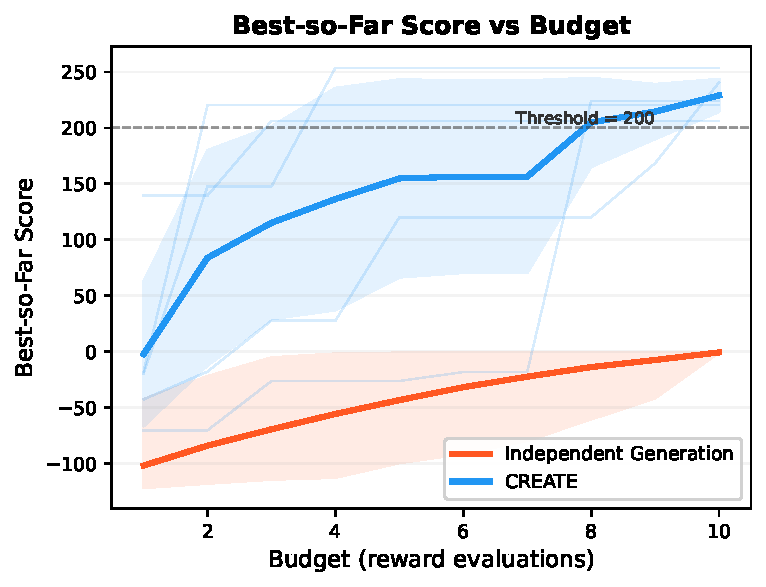
\includegraphics[width=\linewidth]{fig3a_bsf_vs_budget.pdf}
\small (a) Best-so-far score vs.\ budget.
\end{minipage}\hfill
\begin{minipage}[t]{0.32\textwidth}
\centering
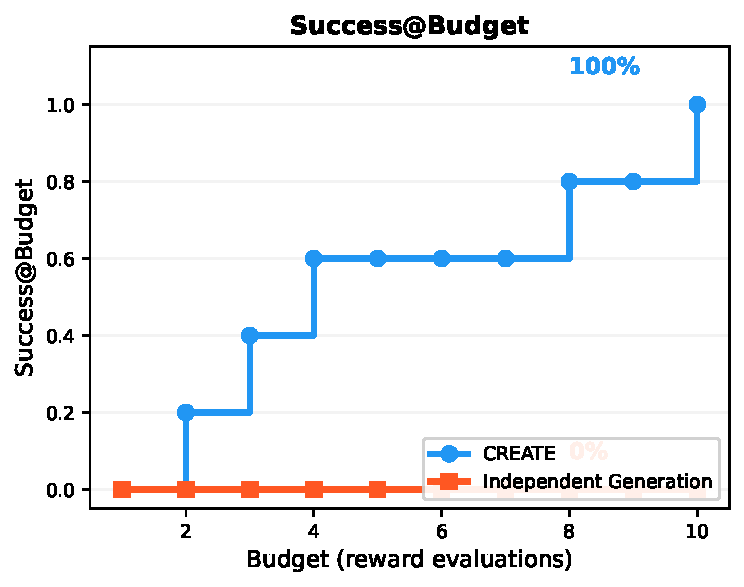
\includegraphics[width=\linewidth]{fig3b_success_at_budget.pdf}
\small (b) Success@Budget.
\end{minipage}\hfill
\begin{minipage}[t]{0.32\textwidth}
\centering
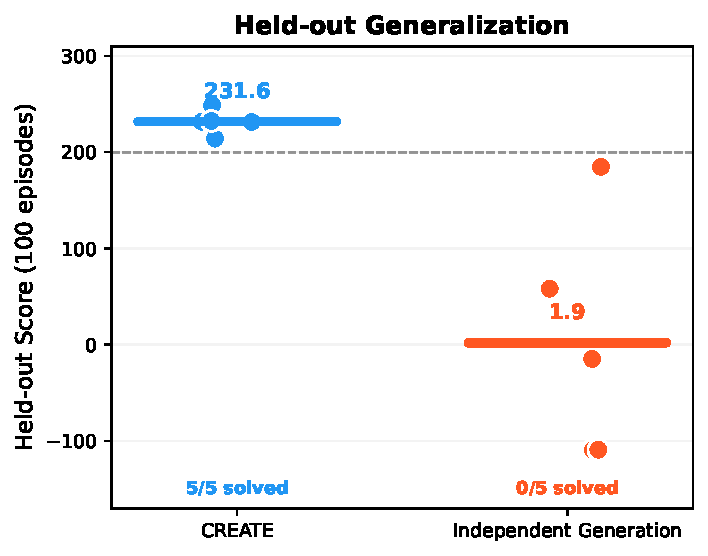
\includegraphics[width=\linewidth]{fig3c_held_out_scatter.pdf}
\small (c) Held-out scores of selected rewards.
\end{minipage}
\caption{LunarLander-v3 search under a common cap of ten reward evaluations per run. Curves carry forward the best-so-far score after a run terminates. Shaded regions: 95\% bootstrap CI (Independent) and $\pm 1.96\,\text{SE}$ (CREATE).}
\label{fig:budget}
\end{figure*}

\subsection{Component Ablation}

Table~\ref{tab:ablation} and Figure~\ref{fig:ablation} report ablations on LunarLander-v3 that isolate the contribution of structured evidence and controlled editing. LLM-once (the five initial rewards) achieves $-2.21 \pm 73.38$, with none reaching the threshold---single-shot generation is insufficient in this task.

\textbf{Coarse Feedback} (2/5) demonstrates that the severity-gated edit controller has inherent search capability even with degraded evidence. Two seeds succeeded (seed 0: 239.52; seed 4: 259.50), indicating that targeted single-component editing can occasionally find correct modifications even when the diagnosis operates on limited information. However, the three failures reveal the cost of imprecise diagnosis. Seed 2 collapsed to $-110.09$: without per-component activation rates and magnitude shares, the reflection agent could not determine whether the problem lay in the progress reward's weight, the stability penalty's mathematical form, or an absent landing bonus---and adjusted the wrong component. This result establishes a gradient rather than a binary relationship: structured evidence does not make iterative editing \emph{possible} (it is possible, unreliably, without it); it makes it \emph{reliable} (5/5 vs.\ 2/5).

\textbf{Unconstrained Refinement} (0/5) reveals the failure mode of non-auditable editing. Two seeds exhibit a peak-then-decline pattern: seed 2 reaches 71.06 at iteration 3 and seed 4 reaches 140.27 at iteration 4, before declining as subsequent multi-component changes destroy previously effective reward structures. Seed 0 gradually improves to 169.90 but cannot close the remaining gap to threshold. When several components change simultaneously, the resulting score change is a compound signal with no per-edit attribution---the system cannot determine which modification was beneficial, neutral, or harmful.

Taken together, the two ablations form a cross-validation. Coarse Feedback (editing intact, evidence degraded) achieves 2/5. Unconstrained Refinement (evidence intact, editing constraints removed) achieves 0/5. CREATE (both components present) achieves 5/5. Neither component alone is sufficient for reliable search.

\begin{table}[t]
\centering
\caption{Ablation results on LunarLander-v3. Five search runs per condition. LLM-once = initial generation without iteration. Coarse Feedback = structured evidence replaced with scalar summary. Unconstrained = intervention tiers and single-component constraint removed. Held-out: 100 episodes, seeds 50000--50099. \label{tab:ablation}}
\resizebox{\columnwidth}{!}{\begin{tabular}{lcccc}
\toprule
Method & Best Dev Score & Held-out Score & Success@10 \\
\midrule
LLM-once & $-2.21 \pm 73.38$ & --- & 0/5 \\
Coarse Feedback & $134.97 \pm 148.43$ & $126.71 \pm 143.85$ & 2/5 \\
Unconstrained Refinement & $114.21 \pm 46.31$ & $102.87 \pm 40.77$ & 0/5 \\
CREATE & $228.98 \pm 16.54$ & $231.63 \pm 12.23$ & \textbf{5/5} \\
\bottomrule
\end{tabular}}
\end{table}

\begin{figure}[t]
\centering
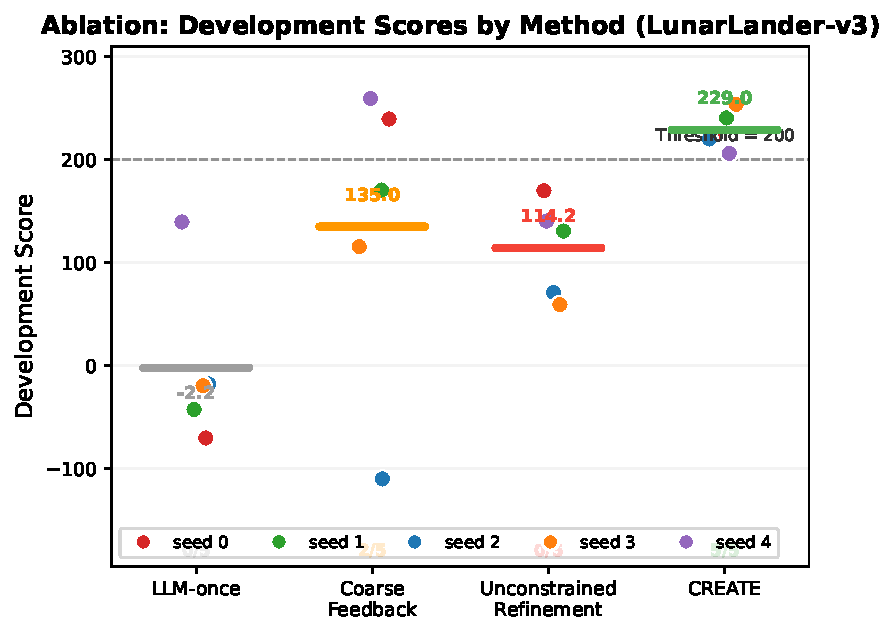
\includegraphics[width=\columnwidth]{fig4_ablation.pdf}
\caption{Per-run development scores for the main ablations on LunarLander-v3. Horizontal bars denote means; dashed line marks the 200-point threshold.}
\label{fig:ablation}
\end{figure}

\subsection{Cross-Environment Validation}

\subsubsection{BipedalWalker-v3}

To assess whether the diagnostic-editing logic transfers beyond discrete-action LunarLander, we applied the identical CREATE workflow to BipedalWalker-v3, a continuous-action locomotion task. All five search paths reached the 300-point threshold (development $311.54 \pm 5.17$, held-out $310.82 \pm 5.03$, 5/5). Table~\ref{tab:cross} summarizes the cross-environment results.

\begin{table*}[t]
\centering
\caption{Cross-environment results. Held-out: 100 episodes, seeds 50000--50099. Evidence roles characterize the statistical strength of each result. \label{tab:cross}}
\resizebox{\textwidth}{!}{\begin{tabular}{lccccc}
\toprule
Environment & Initial Score & Best Dev & Held-out & Success & Evidence Role \\
\midrule
LunarLander-v3 & $-2.21 \pm 73.38$ & $228.98 \pm 16.54$ & $231.63 \pm 12.23$ & 5/5 & Core quantitative \\
BipedalWalker-v3 & $243.26 \pm 70.45$ & $311.54 \pm 5.17$ & $310.82 \pm 5.03$ & 5/5 & Cross-task feasibility \\
Ant-v4 & $-12.04$ & $1414.47$ & --- & 0/1 & Mechanism case \\
\bottomrule
\end{tabular}}
\end{table*}

Four of five BipedalWalker seeds had initial scores already near the threshold (270--290). For these seeds, CREATE applied parameter tuning alone in 2--4 iterations without triggering structural redesign---the edit controller correctly recognized that the reward structure was adequate and limited itself to lightweight adjustments. The fifth seed (seed 4) is a clearer repair case: initial score 103.03, far below the 300-point threshold. Structured evidence diagnosed that the forward velocity reward's mathematical form produced a near-zero activation rate. Component refactoring replaced the sparse binary progress indicator with a continuous forward-velocity signal, and two subsequent parameter-tuning iterations balanced stability and efficiency constraints. The seed reached 304.92 at iteration 3. This repair trajectory---identify component failure, refactor mathematical form, rebalance weights---mirrors the LunarLander repair pattern, suggesting the diagnostic logic transfers across discrete and continuous action spaces.

Held-out evaluation on BipedalWalker shows stronger stability than LunarLander: seeds 1--4 each have held-out standard deviation below 1.0 across 100 episodes, and 498 of 500 held-out episodes terminated successfully at the end of the terrain. The longer episode horizon (approximately 1100 steps) and smoother reward surface of BipedalWalker contribute to this stability.

\subsubsection{Ant-v4 Mechanism Case}

Ant-v4 presents a significantly more challenging test: 27-dimensional observations, 8-dimensional continuous actions, and MuJoCo-based 3D quadruped physics. We conducted a single exploratory run to assess whether the CREATE pipeline can execute in a high-dimensional continuous-control setting, without claiming statistical evidence from a single run.

The initial LLM-generated reward scored $-12.04$. Over eight iterations, the score improved to 1414.47. Structured evidence correctly identified deficiencies in the upright posture maintenance and forward velocity rewards. Parameter tuning improved the weight allocation between forward and upright components, and component refactoring added a height lower-bound gate to prevent ineffective struggling after falls. The final score of 1414.47 is comparable to the reference performance of PPO with the native Ant-v4 reward under the same hyperparameter configuration (approximately 1400--1600), noting that the commonly cited 6000-point threshold for Ant-v4 is based on TRPO and SAC baselines, not standard PPO.

Two additional seeds (seed 2 and seed 3) were run for diagnostic analysis. Across the three seeds, the reflection agent consistently produced correct failure diagnoses at the semantic level---identifying, for example, that an overly aggressive upright gate was suppressing the forward velocity signal (activation rate dropping from 100\% to 44--63\%), or that penalty terms were dominating the sparse progress signal. However, the agent's ability to calibrate the magnitude of its interventions---gate thresholds, penalty coefficients, and weight ratios---did not converge within the available iteration budget. Seed 0 demonstrated that a correctly calibrated repair can reach native-reward-comparable performance; seeds 2 and 3 confirmed that calibration reliability, rather than diagnostic quality, is the current bottleneck in high-dimensional settings. These results characterize the method's current capability boundary and motivate further work on automated coefficient calibration for continuous-control tasks.

\begin{figure}[t]
\centering
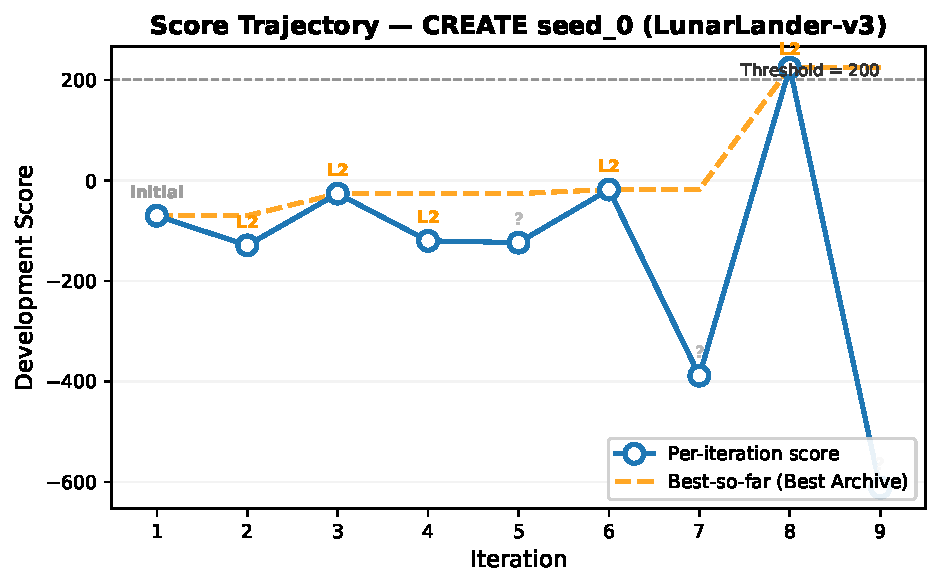
\includegraphics[width=\columnwidth]{fig5a_score_trajectory.pdf}
\caption{Development-score trajectory for CREATE seed 0 on LunarLander-v3. Despite large score fluctuations, the Best Archive preserves the iteration-8 solution (224.21).}
\label{fig:score_trajectory}
\end{figure}

\begin{figure*}[t]
\centering
\begin{minipage}[t]{0.48\textwidth}
\centering
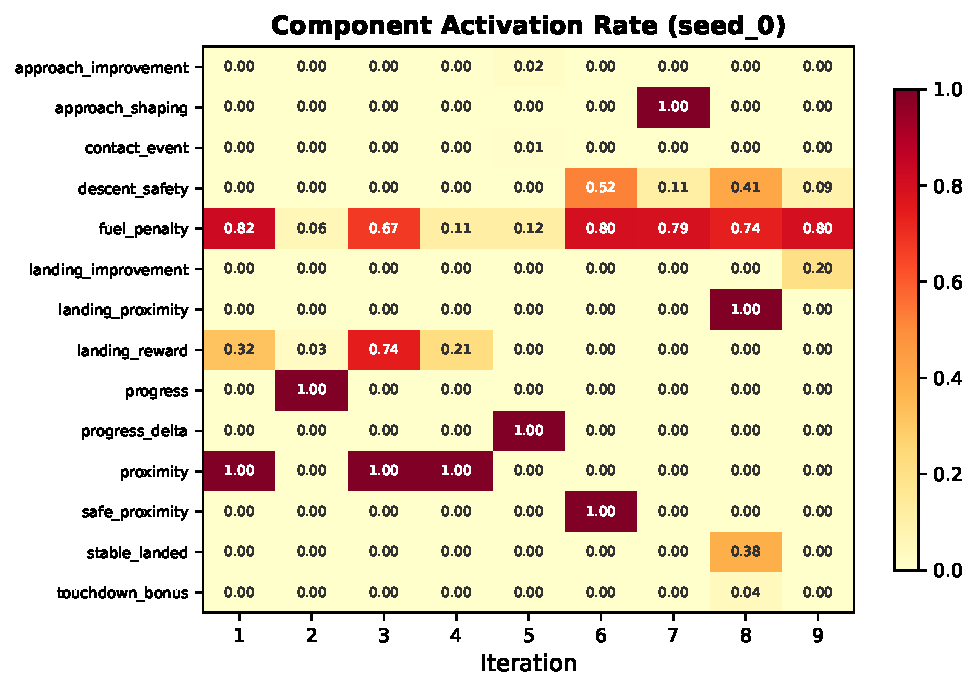
\includegraphics[width=\linewidth]{fig5b_activation_heatmap.pdf}
\small (a) Component activation rates across iterations.
\end{minipage}\hfill
\begin{minipage}[t]{0.48\textwidth}
\centering
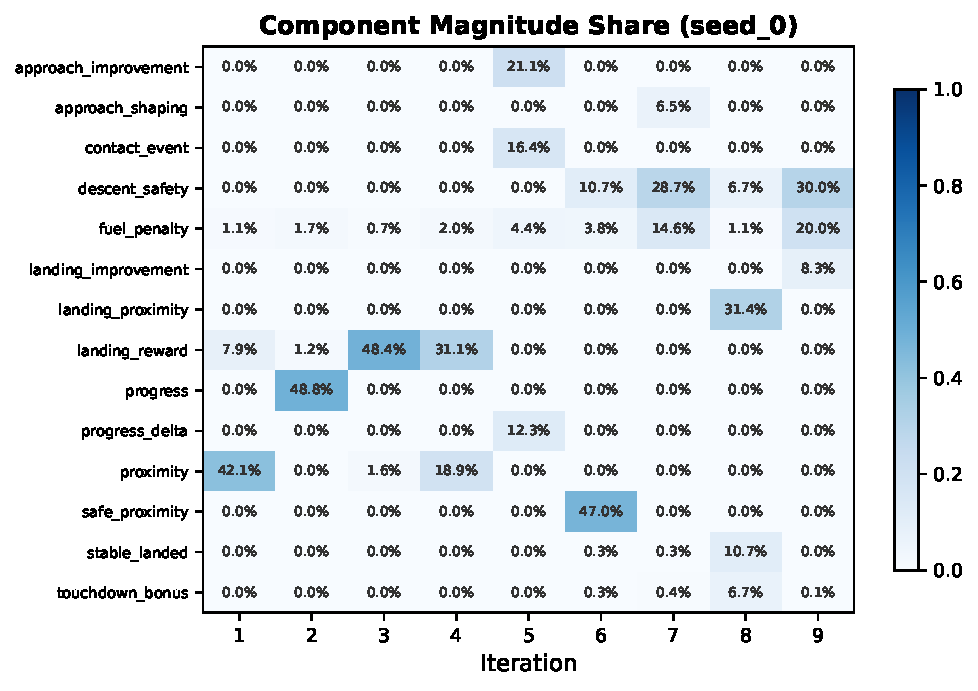
\includegraphics[width=\linewidth]{fig5c_magnitude_heatmap.pdf}
\small (b) Component magnitude shares across iterations.
\end{minipage}
\caption{Component-level diagnostic evidence for CREATE seed 0 on LunarLander-v3. Zero-valued cells include both components with zero activation and components absent from a given reward version.}
\label{fig:diagnostic_case}
\end{figure*}

\begin{figure}[t]
\centering
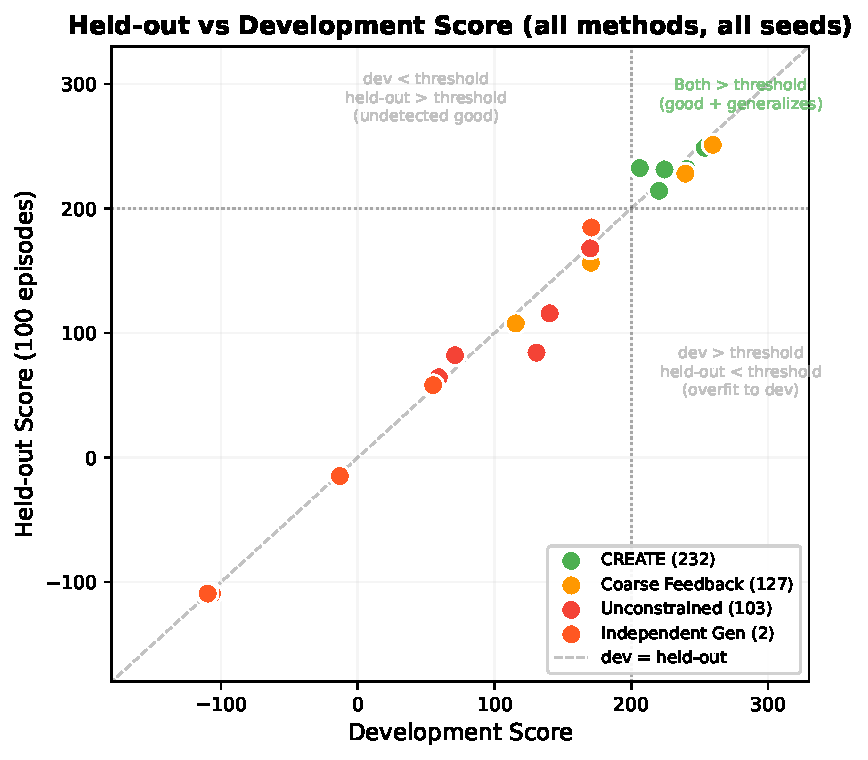
\includegraphics[width=\columnwidth]{held_out_vs_dev.pdf}
\caption{Development versus held-out scores for selected rewards across all methods. Points near the diagonal indicate no systematic shift on the fixed held-out seed set.}
\label{fig:heldout}
\end{figure}

\section{Conclusion}

We studied whether evidence from a completed policy-training run could be used to repair the reward function that produced it, rather than merely to score and discard it. CREATE addresses this question by combining three mechanisms: (1)~component-level evidence that decomposes training outcomes at the granularity of individual reward terms; (2)~auditable failure diagnosis that maps structured evidence to a specific failure hypothesis and editing target; and (3)~a severity-gated edit controller that selects among parameter tuning, component refactoring, and structural redesign, constraining each local edit to one component.

Three findings emerge from the experiments. First, under matched per-evaluation training budgets, iterative single-lineage repair finds high-quality rewards substantially more efficiently than independent candidate generation---5/5 versus 0/5 on LunarLander-v3, with 33 versus 50 total policy trainings. Second, both structured evidence and the controlled-editing mechanism are necessary for search reliability: removing either component causes the majority of search paths to fail. Third, the diagnostic-editing logic transfers across task types: BipedalWalker-v3 achieves 5/5, including a clear repair from 103.03 to 304.92 following the same diagnostic-refactoring-rebalancing pattern observed on LunarLander. An exploratory Ant-v4 run demonstrates that the pipeline can execute in a high-dimensional 3D continuous-control setting, with the generated reward achieving performance comparable to a native PPO baseline; diagnostic quality remains strong in this setting, while coefficient calibration is the primary bottleneck.

These results position structured single-lineage repair as an effective, training-budget-efficient complement to breadth-oriented reward search. When the initial generation success rate is low and training runs produce rich component-level diagnostic signals, the iterative approach reallocates budget from evaluating additional candidates to repairing the current one.

\bibliographystyle{unsrt}
\bibliography{references}

\end{document}
